\documentclass[parskip]{cs4rep}

\usepackage{graphicx}
\usepackage{pseudocode}
\usepackage[T1]{fontenc}
\usepackage{amsmath}
\usepackage{algorithm2e}

\begin{document}

\title{Plan Recognition in RISK}

\author{Jibran Abdus Zaahir Khan}

% to choose your degree
% please un-comment just one of the following
%\degree{Artificial Intelligence and Computer Science}
\degree{Artificial Intelligence and Software Engineering}
%\degree{Artificial Intelligence and Mathematics}
%\degree{Artificial Intelligence and Psychology }   
%\degree{Artificial Intelligence with Psychology }   
%\degree{Linguistics and Artificial Intelligence}    
%\degree{Computer Science}
%\degree{Software Engineering}
%\degree{Computer Science and Electronics}    
%\degree{Electronics and Software Engineering}    
%\degree{Computer Science and Management Science}    
%\degree{Computer Science and Mathematics}
%\degree{Computer Science and Physics}  
%\degree{Computer Science and Statistics}    

% to choose your report type
% please un-comment just one of the following
%\project{Undergraduate Dissertation} % CS&E, E&SE, AI&L
%\project{Undergraduate Thesis} % AI%Psy
\project{4th Year Project Report}

\date{\today}

\abstract{
This paper presents the design and implementation of a plan recognition agent based on an algorithm published by Christopher Geib and Robert Goldman in 2009[ref to work] called The Probabilistic Hostile Agent Task Tracker (PHATT). The plan recognition agents goal is to attempt to infer the unknown plan of a player from observations of their behaviour in the RISK environment.
}

\maketitle

\section*{Acknowledgements}

(Distinguish between academic and non-academic work.)

\tableofcontents

%\pagenumbering{arabic}

\chapter{Introduction}

\begin{flushleft}
\textit{AI has the potential to become the new driving force behind computer game innovation.}
\end{flushleft}
\begin{flushleft}
John David Funge, Artificial Intelligence for Computer Games
\end{flushleft}

\section{Motivations}

\subsection{What is game AI}

The application of Artificial Intelligence techniques to games has been an area of research ever since the beginning of significant work on A.I. Presently termed game A.I. it is a term used to differentiate A.I. applied in games from academic AI, and though the techniques have typically come from academia it is significantly different in both its scope and application.

\subsection{Difference between academic and game AI}

As the primary goal of academia is to further human understanding the scope of developed A.I. techniques are preferably general in application. Game A.I. on the other hand is built to create the illusion of intelligence and provide good game play for those playing the game, it therefore needs not be as and is built with a singular purpose in mind which is usually considered to be any kind of control problem in a game.

Reference - difference between academic and game A.I [AI and computer games]

\subsection{Computer Graphics previously getting more attention}

Companies in video games industry tirelessly look for an edge over their competition. This edge has typically come from computer graphics, effects such as dynamic rendering, the move from two dimensional to three dimensional to keep their customers interest. 

\section{AI getting more attention now}

What is emerging is the idea that as users become accustomed to high quality graphics, developers will need something new to give their product an edge over their competitors. That edge will hopefully be better quality game A.I.

Mention notable A.I's like F.E.A.R.

With this shift in focus, there is a greater incentive for the continued development of more sophisticated game A.I. likely with techniques developed in academia. The application of plan recognition algorithms may provide such an opportunity. 

\section{Plan Recognition}

Plan recognition definition.

When research began

\section{Applications of Plan Recognition}

How it is used

Currently plan recognition applications range from computer security to help systems (more detail).

\section{Application of plan recognition algorithms to games}

Plan recognition can perform automated game analysis which can be used by players to improve their performance. 

Plan recognition can lead to AI responses that are personalized.

\section{Artificial Intelligence and Board Games}

In 1915 Leonardo Torres y Quevedo's built a chess automaton[ref]. It was considered the worlds first computer program and arguably the beginning of Artificial Intelligence and board games.

Thirty five years later Alan Turing published a landmark paper[ref], marking what many consider to be the 'birth of Artificial Intelligence'. Soon after John McCarthy officially coined the term Artificial Intelligence at a conference in Dartmouth College[ref]. He defined it as "the science and engineering of making intelligent machines"[ref].

E.g
There existed Christopher Stracheys Game AI for the board game draughts built in 1951[ref]. As AI continued to develop so did the complexity of the A.I's seen in computer games, first AI to appear which used enemies was arcade game [ref].

Since then notable achievements such as Garry Kasparovs defeat to IBMs chess computer Deep Blue in 1997 [ref] have continued to impress the public. 

From history it seems clear that AI and its application in games are intertwined becoming a growing area of interest in both commercial and academic fields.

Games are often considered a good metric for testing the quality of an AI [Ref].. 

Some academic work done on RISK in particular. Development of an Intelligent Artificial Player for the Game of Risk[ref]. The author Michael Wolf[ref] claims RISK is generally well known but under recognised by academia.

\section{Aims}

What do we want to achieve?

An aim is a general statement of intent. It describes the direction in which the learner will go in terms of what they might learn or what the teacher/training will deliver.

To design a plan recognition agent for the board game RISK based on the PHATT algorithm developer by Geib and Goldman.

To implement a plan recognition agent for the board game RISK that can make successful predictions.

To further understanding of the complexities of performing plan recognition in the board game RISK.

\section{Objectives}

An objective is a more specific statement about what the learner should or will be able to do after the training experience.

To show plan recognition algorithms can be used successfully to predict an agent's plan in the board game RISK.

To provide insight into the complexities of creating a plan recognition mode for the RISK environment.

To build a plan recognition agent that has an accuracy better than randomly picking a mission card.

To provide insight into the nature of making plans in RISK. 

\section{Hypothesis}

What do you want to answer?

Are plan recognition algorithms beneficial in games? Specifically RISK?

If the probability of a mission card is the highest among all the other mission cards of an agent, then it will be the correct mission card.

The predictions of the winners will be better than that of lowers.

Why because they are an artificially derived benefit which can be used by a player to optimize their behaviour, not solely , but in conjunction with the results of a plan recognition system.

Using more data from risk environment in the computation of the likelihood of explanations, the better the prediction accuracy will be.

\section{Paper Structure}

The structure of the paper is as follows:

The following chapter presents a background to the project where plan recognition and the board game RISK are introduced. Reasons for using plan recognition in board games are then discussed.

Chapter 3 describes the methodology of the project, it is split into two sections. The first is design, in this section PHATT is introduced and the design of the plan recognition agent is detailed. The subsequent section is implementation. Code related issues such as modifications to the open source project and any relevant design concepts are discussed. 

Finally there is the evaluation and conclusion chapters. In these the experimental findings are presented and discussed and any conclusions derived from the experimental findings are presented.

\chapter{Background}

\section{Previous Work in Plan Recognition}

Many consider one of the earliest projects on plan recognition to have been in 1978. Schmidt et al [ref - Schmidt Plan Recognition Problem] had conducted experiments to determine whether or not people inferred the plans of other agents. From their results they created a rule based system called BELIEVER which attempted to capture the process of plan recognition. 

Three years later Cohen, Perrault and Allen identified two different types of plan recognition \textit{keyhole} and \textit{intended} [ref - cpa strategies in natural language processing]. 

They defined each as:

\begin{itemize}
\item
\textit{Keyhole plan recognition} is the recognition of an agent's plan through unobtrusive observation".
\item
\textit{Intended plan recognition} is the recognition of the plan of a cooperative agent who wishes to be understood.
\newline
\end{itemize}

In 1986 Kautz and Allen published a paper titled "Generalized Plan Recognition"[ref] which set the frame work of many plan recognition projects that followed and formed the basis of plan recognition through logic and reasoning. They defined keyhole plan recognition as involving the identification of a set of top-level goals from possible plans, which could be decomposed into related sub goals and basic actions, thus creating an event hierarchy also known as a \textit{plan library}. 

It was Charniak and Goldman[ref - 1991 paper] who first argued that plan recognition was largely a problem of reasoning under uncertainty and that any system which did not account for uncertainty would be inadequate. They went on to propose a probabilistic rather than logic based approach to  plan recognition using a Bayesian model. Their research continues to be popular (check statement?) in many avenues of research including its application in games.

Albrecht, Zukerman and Nicholson [ref 1998 A Bayesian model for keyhole plan recognition in an adventure game] performed research on keyhole plan recognition using dynamic Bayesian networks to represent features of an adventure game. The result of their experiments they claimed "showed promise" for some domains. 

More recently Synnaeve and Bessiere [ref - RTS Bayesian model plan recognition in Starcraft 2011] published a paper of the design and implementation of a plan recognition agent that through observations of building construction in the game Starcraft, can predict the types of units a player intends to produce based on what buildings they construct.

\subsection{An Example of Plan Recognition}

We can introduce common concepts, assumptions and the process of plan recognition with an example of an agent attempting to infer the plan of another agent in a non-adversarial environment. 

Person A is cooking a meal for Person B, in other words A has a single \textit{root goal} (a state they wish to reach), such as cooked beef hamburgers. This root goal can be decomposed into a number \textit{sub goals} of such as cook meat patties or \textit{actions} such as make meat patties  which can be further decomposed into single actions

A wanting to surprise B, will not tell B what his root goal is. B cannot know what A is thinking but B must then somehow infer what A's root goal is likely to be by \textit{observing} A cook in this way A's behaviour can be modelled as a Hidden Markov Model. Person B then models A's plan as follows. 

Person B assumes A is a rational person, and that A has a \textit{plan} to achieve this root goal. Whatever A's root goal is, it can likely be decomposed into \textit{sub goals} such as cook hamburger meat. These sub goals can then be broken down into basic \textit{actions} to achieve those sub goals, such as take hamburger meat out of packet. An important point to note is that these basic actions are not limited to only being part of a sub goal.

To simplify this example, let us make some assumptions:

\begin{itemize}
\item
A believes that they can cook a meal.
\item
B can only infer the cooking plan of A by observing what A is cooking.
\item
B knows everything that A can cook.
\item
Through observing A cook, B can predict with absolute certainty what A will cook.
\item
A cannot hide any observations.
\item
A only wishes to cook one meal.
\item
A has no preferences of what to cook, in other words given a choice the probability of choosing is equally likely.
\item
One A does not change cooking plan.
\end{itemize}

Given these assumptions and B's knowledge of A's cooking abilities we can model a \textit{plan library}, which is the set of all of A's possible cooking plans in the decomposed form that was previously detailed.

\begin{figure}[h]
\centering
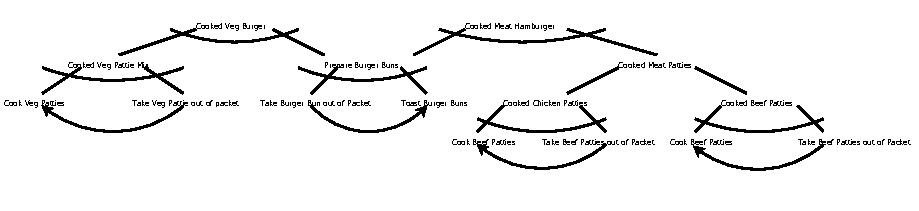
\includegraphics{images/example-plan-recognition}
\caption{Root goals are located at the top, sub goals are in middle. and-nodes are represented by an undirected arc across the lines connecting the parent node to its children, or-nodes do not have this arc. Actions or goals that are dependant on a previous action are represented by an arc with an arrow.}
\label{fig:example-plan-library}
\end{figure} 

The top level goals or root goals are cooked vegetarian (veg) burgers and cooked beef burger. These root goals can be broken down into sub goals, for the case of cooked veg burger the sub goals are cooked veg pattie mix and prepare burger buns.

A takes bread out of its packet and toasts the burger bun, looking at the plan library we have two possible \textit{explanations} for As behaviour, cooked veg burger or cooked beef hamburger.

Each of these explanations are equally likely at this point.

A takes the meat of the packet, now given our assumptions we can conclude that A's plan is too cook beef hamburgers. At this point B can conclude that they will be getting a ham burger for dinner.

\newpage

\section{Introduction to RISK}

Developed and released by french director Albert Lamorisse in 1957 as La Conqu\^ete du Monde, RISK is a turn-based board game for two to six players. There exist many variations but the standard version, which this paper is concerned with, is an adversarial environment where players vie to control a fully observable board portraying a static geographical map of the Earth.

\subsection{Equipment}

\begin{figure}[h]
\centering
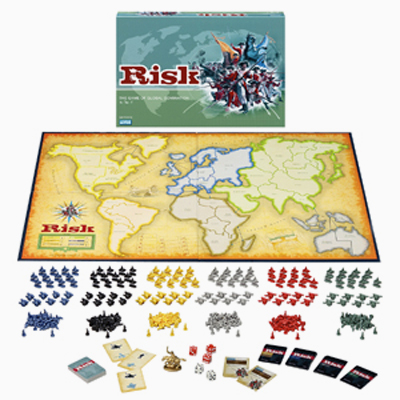
\includegraphics{images/risk-board}
\caption{Risk Equipment}
\label{fig:risk-equipment}
\end{figure}

The game consists of three pieces of equipment:

\begin{itemize}
\item
A board portraying a geographical map of the earth.
\item
Different coloured tokens called \textit{armies}.
\item
Two sets of regular six-sided dice.
\end{itemize}

\subsection{Rules}

Games are played following a set of rules which define the purpose of each piece of equipment and how they relate to each other. The following is a brief summary of these rules.

The board is divided into forty two \textit{territories}. Each territory is a representation of a real country on Earth. These territories are partitioned into six \textit{continents} usually corresponding to their real continent grouping.

Armies are placed in countries. If a player places an army in a territory, this declares that the player \textit{occupies} that territory. Players must have at least one army placed in a territory they own at all times. Players can then choose to place as many additional armies as they wish in that territory.

How a player wins largely depends on the \textit{Game mode}. Game modes significantly impact the behaviour of players and is decided by players beforehand. In standard RISK they are:
\newline

\begin{tabular}{|l|p{11cm}|}
\hline 
\textbf{Game Mode} & \textbf{Description} \\ 
\hline 
Domination & Players aim to conquer a certain number of territories, \\ 
\hline 
Mission & Each player is given a single unique mission card. A mission card describes a state they must reach e.g. Occupy North America and Africa, for the rest of the game this is their \textit{root goal} which only they know. In order to win they can either complete this root goal or eliminate all other players. \\ 
\hline 
Capital Risk & Each player is given a Capital territory and to win a player must capture all other Capital territories. \\ 
\hline
\end{tabular} 
\newline

This paper is concerned with the mission game mode \textbf{only}, therefore the following sections describe rules only for that game mode.

After an initial setup, each player's turn is split into three distinct phases which always occur in the same fixed order. These phases are:

\begin{enumerate}
\item
Reinforcement
\item
Attack
\item
Movement
\newline
\end{enumerate}

In each phase a player performs atleast one discrete \textit{action} which helps to further the players goals, thus forming a sequential task environment.

\subsubsection{Initial Setup}

The game begins with an an initial setup, it involves:

\begin{itemize}
\item
Territories being divided equally between players.
\item
Players being given a starting number of armies which is inversely proportionally to the number of players.
\item
Players distributing their starting armies over their territories.
\item
Each player being given a mission card.
\end{itemize}

\subsubsection{Reinforcement Phase}

At the start of a player's turn, they receive \textit{reinforcements} in the form of additional armies. The act of placing an army in a territory is called \textit{reinforcement}.  The number of additional armies received is based on the number of territories a player occupies and whether they occupy any continents.
\newline

\begin{table}[ht]
\centering
\begin{tabular}{|c|c|}
\hline 
\textbf{Occupied Continent} & \textbf{Number of Bonus Armies} \\ 
\hline 
Asia & 7 \\ 
\hline 
North America & 5 \\ 
\hline 
Europe & 5 \\ 
\hline 
Africa & 3 \\
\hline
Australia & 2 \\
\hline  
South America & 2 \\
\hline 
\end{tabular}
\caption{Occupied Continent Army Reinforcement Bonus}
\label{table:continent-bonus}
\end{table}

\subsubsection{Attack Phase}

Once a player has distributed their armies from the reinforcement phase, they can choose to \textit{attack}. 

Territories occupied by a player that contain more than one army can attack adjacent territories occupied by any other player. An attack consists of several \textit{battles}. The outcome of a battle is decided by means of rolling two sets of dice, thus making it a stochastic environment. One set is rolled for the \textit{defender} of the territory and the other for the \textit{attacker}. 

The number of dice each player receives for a battle is dependant on the number of armies placed in each of the players respective territories. The defender receives a die per army up to two armies. The attacker receives a die per army upto three armies not including the single army they are required to have in that territory while occupying it. 

The general rules of engagement are, dice rolls of each player are compared on a one to one basis in descending order of values. The player with the lower value at each comparison loses a single army, if the die are equal the attacker loses an army. The number of comparisons per battle are set by the number of dice the defending player has rolled. The attacking player can commence as many battles as they wish during an attack provided they have more than one army in the attacking territory.

An attack of a territory has three outcomes:

\begin{itemize}
\item
A \textit{failedAttack} by the attacker as they have only one army remaining in which case they must retreat and a \textit{successfulDefence} by the defender who retains the territory.
\item
A \textit{failedAttack} by the attacker as they choose to retreat before having only one army remaining and a \textit{successfulDefence} by the defender who retains the territory.
\item
A \textit{successfulAttack} by the attacker who occupies the territory and a \textit{failedDefence} by the defender who has no armies remaining and so loses the territory. The attacking player, leaving atleast one army behind, must then move armies from the territory they attacked from into the newly occupied territory.
\end{itemize}

A player can perform any number of attacks from any territory they own during their turn, provided they have more than one army in the territory they choose to attack from.

\subsubsection{Army Movement Phase}

When either the player chooses to end the attacking phase or can no longer attack because they do not occupy a territory which contains more than one army their movement phase begins.

During their movement phase a player may move armies from one territory to an adjacent territory they own, provided they leave atleast one army in the territory the armies were moved from. This action can only be done once per turn in this phase, after which the movement phase is finished.

After the movement phase has been completed the players turn ends and another players reinforcement phase begins.
\newpage

\section{Why Plan Recognition in Board Games}

Algorithmic landmark - such as the solution of the game of checkers 

In the realm of board games such as chess, there have for many years dominated a number of algorithms such as the:

Minmax Algorithm with Alpha-Beta Pruning

Many games today have a large number of alternative moves are stochastic and have hidden state attributes. "Applying traditional game tree search algorithms designed for perfect information games that act on the raw state representation is infeasible" [ref Monte Carlo Planning in RTS Games], this has been said because the search space for such games is large and that finding the best move would take an unreasonable amount of time (Find a ref for this)

Instead of a brute force method of finding the best alternative the idea of plan recognition offers another method. Use plan recognition algorithms one can weed out unlikely explanations before committing to a search of the 

Main benefit is that responses can be personalized.

This issue prompted research into the development of variants of the original algorithms that could cope but this 
Using these algorithms people like Kabanza are starting to be able to tackle certain aspects which are harder to model?

\chapter{Methodology}

\section{Design}

\subsection{Introduction to PHATT}

PHATT was published in 2009 by Geib and Goldman. In their paper they presented the central realization of the PHATT approach being "that plans are executed dynamically and the actions that an agent takes at each step depend critically on the actions he has previously taken". 

They went on to introduce a model of plan execution based on the notion of \textit{pending sets} of actions. They defined a pending set as the actions an agent could take based on the actions that the agent had already performed, calling it "actions that are pending execution by the agent".

In summary, plan execution according to PHATT was modelled as the following process. An agent would first choose a goal, then a set of plans to achieve that goal. Any actions of those plans that had no pre-requisite actions would form the initial pending set of the agent. The agent would then perform an action from the initial pending set. This would result in some actions being added to the pending set and others being removed to form a new pending set. The agent would then continue to perform actions until

Following their new model of plan execution Geib and Goldman proposed an algorithm utilizing a Bayesian approach to perform probabilistic plan recognition. It computed \textit{Pr(g}|\textit{obs)}, the conditional probability of a goal \textit{g} given a set of observations \textit{obs} by computing \textit{Pr(exp}|\textit{obs)}, the conditional probability of a particular explanation \textit{exp} of the likelihood of an agent having that root goal, given a set of observations \textit{obs}.

Using Bayes Rule they defined \textit{Pr(exp}|\textit{obs)} as:\newline

\centerline{
\textit{Pr(exp}|\textit{obs)} = \textit{Pr(exp} $\wedge$ \textit{obs)} / \textit{Pr(obs)}
}

They then (as other practical Bayesian systems do) exploited the equivalent formulae\newline

\centerline{
\textit{Pr($exp_0$}|\textit{obs)} = \textit{Pr($exp_0$} $\wedge$ \textit{obs)} / $\displaystyle\sum\nolimits_{i}$ \textit{Pr($exp_i$} $\wedge$ \textit{obs)}
}

This they described as the conditional probability of the specific explanation $exp_0$ being computed by dividing the probability of that explanation and the observations by the sum of the probability mass associated with al of the possible explanations.

For an exact specification of PHATT and its probability model please refer to [ref].

\subsubsection{Computing an Explanation's Probability}

To go on to compute \textit{Pr(exp} $\wedge$ \textit{obs)} according to Geib and Goldman's paper, requires three probabilistic features:\newline

\begin{itemize}
\item
The probability of the root goal.
\item
The probability of choosing each sub goal.
\item
The probability of picking an action from the pending set.\newline
\end{itemize}

Each of these features are multiplied together in the following manner:\newline

\centerline{
\textit{Pr(exp} $\wedge$ \textit{obs)} = \textit{P}(\textit{goals})\textit{P}(\textit{plans}|\textit{goals})\textit{P}(\textit{obs}|\textit{exp})
}

The probability of a given explanation is then calculated by multiplying together the priors for each goal, the probabilities of each of the sub goals, and the probability of the observed actions being chosen.

For a full specification of how to compute an explanation probability please refer to [ref]

With an idea of the operation of PHATT now in mind it is now necessary to design PHATT to operate in RISK.

\subsection{Environment Modelling}

For PHATT to operate in RISK, modelling of the RISK environment is necessary. This process began with the identification of the root goals, sub goals and actions in the RISK environment as these would constitute the three probabilistic features necessary by PHATT.

\subsubsection{Root Goals}

The root goals of this environment are the mission cards, these are:

\begin{itemize}
\item
Occupy Europe, Australia and one other continent.
\item
Occupy Europe, South America and one other continent.
\item
Occupy North America and Africa.
\item
Occupy North America and Australia.
\item
Occupy Asia and South America.
\item
Occupy Asia and Africa.
\item
Occupy 24 territories.
\item
Occupy 18 territories and occupy each with atleast two troops.
\item
Eliminate a player.
\newline
\end{itemize}

The above list all the mission cards from the RISK environment, due to the modelling choices which will be presented later, a subset where the mission involved conquering continents were focused on as due to the high level of overlap other missions which would likely hamper predictions.

As mission cards are handed out to players' at random, the prior probability of each root goal is 1/\textit{N} where \textit{N} is the number of mission cards.

\subsubsection{Sub Goals}

For root goals that involve occupying atleast two continents it follows by definition that the sub goals of that root goal is occupying each continent. Two root goals allow an option to occupy a continent of choice provided they also occupy two particular continents. These two types of root goals therefore make the occupation of any single continent part of atleast one mission card.

\subsubsection{Actions}

In RISK the key actions players perform are:

\begin{itemize}
\item
Attacking a Territory.
\item
Defending a Territory.
\item
Occupying a Territory.
\item
Losing a Territory.
\item
Reinforcing a Territory.
\item
Moving armies into a Territory.
\newline
\end{itemize}

Each of these must be modelled in a manner that contributes towards explanations of the players behaviour.

\textbf{Attacking and Defending}

The actions of attacking and defending a territory only ever occur together and so given the outcomes of a battle, the actions of attacking and defending can be modelled as consistent or inconsistent towards achieving a root goal as follows:

SuccessfulAttack - the best indication of a player intention

FailedAttack - is a clear message of the intention of a player to occupy that territory and therefore should be considered a consistent action though given a less weight than that of a successful attack due to the nature of success and failure.

SuccessfulDefence - another good indication of 

FailedDefence - inconsistent because a player would successfully defend 

\textbf{Fortify}

To \textit{fortify} a territory is the act of placing an army in a territory. The fortify actions that a particular player $p$ can perform at any turn $t$ is based solely on the territories that $p$ owns during turn $t$. The pending set of any player for the fortify actions is therefore modelled as follows. 

For each territory $T$ that $p$ owns at a certain turn $t$. In $p$'s pending set is an action to fortify $T$. If a territory $T_{new}$ is lost by $P$ (it is attacked and then occupied by another player), its corresponding fortify action is removed from the players pending set for turn $t+1$. Conversely if another territory $T_{other}$ is gained by $P$ then a fortify action for $T_{other}$ is added to the players pending set at turn $t+1$.\newline

\textbf{Movement}

Initially the movement model was based on the attack model where the smaller the number of actions the bigger the weighting should be, this is an incorrect model as the number of territories a player owns increases as a player gains more consistent movement and reinforce actions as they continue to be successful in their goal.

The new model worked in such a way:

Probability model changed to proportion of consistent actions * 0.1 
0.9 - proportion for consistent probability
1 - proportion for inconsistent probability

Due to time constraints did not use it. Why?

Movement is the action of moving armies from one territory to another adjacent territory.

Pending set for move is neighbouring countries where a player has more than one army.

From an analysis of the environment model, it allowed for a formal definition of its various data structures

Capturing effectively the impact of movement of armies to a Territory 
A list of available attack actions are created for each player and based on what they do a probability is calculated.\newline

\subsubsection{Explanations}

An explanation must be designed to contain all the necessary data required to compute its probability.

It therefore must contain these features:

A name
A list of root goals
A list of method choices
A list of consistent actions
A list of inconsistent actions

One may ask that why store inconsistent actions, the model, some actions are not defence actions of a territory that is not in the mission is not inconsistent but would be if we where to use a blank if not consistent then inconsistent AND why include inconsistent actions because there is less overhead than having to search through an entire list of actions

RG is the root goal
MC is method choice
CA is consistent action

Explanation data structure is $E$ = \{ explanationName, RL, ML, CA \}

Given the list of root goals and sub goals, the full list of explanations that will be considered are:

\begin{itemize}
\item
Occupy Europe, Australia and Africa.
\item
Occupy Europe, Australia and North America.
\item
Occupy Europe, Australia and South America.
\item
Occupy Europe, Australia and Asia.
\item
Occupy Europe, South America and Asia.
\item
Occupy Europe, South America and Africa.
\item
Occupy Europe, South America and North America.
\item
Occupy Europe, South America and Australia.
\item
Occupy North America and Africa.
\item
Occupy North America and Australia.
\item
Occupy Asia and South America.
\item
Occupy Asia and Africa.
\newline
\end{itemize}

Each of these are considered as possible explanations of a players behaviour.

\subsubsection{Territory}

As territories contribute to several different sub goals they require a model. The data structure of a territory contains a number of important items.

The name of the territory
The actions available by owning this territory.

(Diagram of territory and associated actions)

C = Territory Object

In the form of the pending set of that Territory and the countries name C = { TerritoryName, PS }

By owning a Territory a player can perform a number of actions.
Each Territory is modelled as a state. Each state has a number available actions which together form its associated pending set. \newline

\subsubsection{Continent}

Each continent C contain several territories T. Therefore the data structure is a tuple of the name of the continent and the set of territories that are contained in that continent.

C = {continentName, <T1... Tn>}

\subsubsection{Player}

The term \textit{Player} can be used inter changeably with the term agent that was introduced in previous descriptions. A data structure of a player must contain a number of things:

Each player has a list of countries they own.
Each player has a name.
Each player must have a history of active pending sets.
Each player must have a list of actions they have taken.
Each player must maintain a list of explanations that has been assigned to them.

Each player must be manageable.

The active pending set of an agent is decided \textit{a priori} based on the territories a player owns.

\subsection{Issues Applying PHATT to RISK}

NOT COMPLETE

Another difference is that I do not store or manipulated derivative trees as the original paper includes in the pseudo code it presents, this is due to hard coding derivative trees into explanations.

Main change is that PHATT works in an action space whereas I have had to adapt the implementation to represent the state of the 'risk world' for the algorithm to operate.

For each player a 

\subsubsection{Building the Set of Explanations}

In building the set of explanations there is in this design a difference. Where the 

\subsection{Prediction Agent Pseudo Code}

In this section is presented the pseudo code of the most significant operations of the plan recognition agent.

\subsubsection{Explanation Allocation}

Given a list of all explanations \textit{EL} which contain all the explanations for an environment $E_1$ $\dots$ $E_j$, and a list of observations $\sigma_l$ which contain all the observations of a player in the environment $\sigma_1$ $\dots$ $\sigma_n$.  A player is then allocated a number of explanations of their behaviour.

\begin{pseudocode}{ExplanationAllocation}{\sigma_1 \dots \sigma_n}
\begin{algorithm}[H]
\ForAll {E $\in$ EL}{

	\ForAll{$\sigma$ $\in$ $\sigma_l$}{

		\If {$\sigma$ is consistent with E \textbf{AND} E has not already been added}{

			add E to AE
		}
	}
}
\end{algorithm}
\end{pseudocode}

The pseudocode above is a nested loop. First it loops through each explanation $E$ in the list of all explanations $E_l$, then during the first loop again loops through each observation $\sigma$ in the list of observations $\sigma_l$. 

At each point in the loop through the observations two conditions are checked. The first condition \textit{observationIsConsistent} is a method which  returns true if and only if the current observation is contained in the list of actions that are consistent with that explanation \textit{E}. 

The second condition returns true if only if the explanation is not already in the list of that agents explanations \textit{AE}.

\subsubsection{Explanation Computation}

To compute the probability of an explanation, first a function that generates all the available actions a player can perform is required.

\begin{pseudocode}{GeneratePendingSet}{-}
\begin{algorithm}[H]
\textit{newPendingSet} = $\emptyset$

\ForAll {T $\in$ AT}{

	addAction(FortifyT) to \textit{newPendingSet}\newline
	addAction(LoseT) to \textit{newPendingSet}

	\ForAll{N $\in$ T}{
			
		\eIf {playerOwnsN}{

			addAction(MovementT) to \textit{newPendingSet}
		}{

			addAction(OccupyT) to \textit{newPendingSet}
		}
	}

	\Return{newPendingSet}
}
\end{algorithm}
\end{pseudocode}

After initializing an empty \textit{newPendingSet} which is a data structure that can only contain performable actions in the environment. The above pseudo first loops through each territory \textit{T} in the list of all the territories \textit{AT} that a player owns. For each territory a \textit{FortifyT} action and a \textit{LoseT} action is added to the newPendingSet. 

Before proceeding onto the next territory another loop is done through the list of neighbours \textit{N} of that territory with a simple if-then-else statement. If the player owns that territory a \textit{MovementT} action is added to the newPendingSet, if not then a \textit{OccupyT} action is added to the newPendingSet, at the end the newPendingSet is returned and can be cached if necessary.

\begin{pseudocode}{ComputeExplanation}{-}
\begin{algorithm}[H]

\textit{expProbability} = 1.0

\ForAll {R $\in$ RGL}{

	\textit{expProbability} = \textit{R} * \textit{expProbability}	
}

\ForAll {S $\in$ SGL}{
	\textit{expProbability} = \textit{M} * \textit{expProbability}
}

\ForAll {O $\in$ OL}{
	\textit{expProbability} = \textit{computeObservationProbability(O)} * \textit{expProbability}
}

\Return{explanationProbability}
\end{algorithm}
\end{pseudocode}

The above pseudo code details the computation of an explanation. After initialising the float \textit{explanationProbability} three loops are performed. The first loop multiplies each of the root goal probabilities $R$ with explanationProbability. The second loop multiplies each of the sub goal probabilities $S$ by explanationProbability. Using the method computeObservationProbability, the last loop computes the probability of choosing each observation $O$ by the player from the list of observations $OL$.

The computeObservationProbability method is a vitally important operation as it computes one of the three probabilistic features required by the algorithm.

\subsubsection{Equal Distribution}

NOT COMPLETE

This is where each feature of an explanation is modelled as equally likely amongst its alternatives. 

\subsubsection{Simple Weighted Distribution}

NOT COMPLETE

Following an idea found from an earlier paper by Geib[ref] which proposes a weighting towards consistent actions [ref - new model of plan recognition] that contribute to a plan. A different method of assigning probabilities to pending set actions was deduced.

Actions are separated into consistent and inconsistent actions. A hard coded weight is then equally distributed between each action.

\subsubsection{Proportional Weighted Distribution}

NOT COMPLETE

Write up explanation of new method of probability distribution.

\subsubsection{Explanation Evaluation Stage}

For each agent
For each agents explanation choose the highest probability.

\subsection{Example of Operation}

Use example written up before.

\subsection{Conceptual Issues}

Narrowing large search space
Initially the model was based on the plan library proposed in the PHATT paper. This was not good therefore utilized the constraints of countries to narrow the number of possible explanations and actions?

Calibrating Mechanisms of algorithm
Uniform distribution
Simple weighting based on reasoning about implications of an action to an explanation
Weighting based on number of consistent and inconsistent actions available to a player when an action is performed.

Manual Simple Weighting
Positively weighted probabilities towards consistent actions and negatively towards inconsistent actions

Initially had a simple system of choosing a weight to distribute

\subsubsection{Probability Assignment}

Finding
Equal Distribution does not work very well for simple explanations

so made up:

Weighted Distribution based on consistent and inconsistent actions

Though question is How to assign weights to consistent and inconsistent actions?

Total number of actions are counted, and are separated into inconsistent actions and consistent actions and a weight is split among inconsistent actions and consistent actions. Problem is that it seems this system is too sensitive.

Because of sensitivity had to make up a more evenly weighted automatic system.

\subsection{Summary}

\section{Implementation}

\subsection{Modifications to Open Source Project}

Initialised plan recognition agent and processing class within 

Initialisation of plan recognition agent and processing class in risk game.

Code that injected events into processing which passed it to the plan recognition agent in various places namely:

\begin{itemize}
\item
Player Initialisation
\item
Player Removal
\item
Territory Occupation
\item
Attacks
\item
Army Movements
\end{itemize}

\subsection{System Construction}

The architecture of the plan recognition agent was built around an existing open source RISK game developed by Yura Mamyrin (verify name) and (anyone else) in (year?)[ref - to website?].

Initially the architecture was designed as a distributed system where the system would store its own subset of data structures from the RISK environment.

Agent data was generated such as countries they owned.
Agent explanations computed by the plan recognition agent based on events from the environment.

The reason for this choice was the simplicity of its implementation at the time.

(Diagram of data structure of local copy)

Adding data to this hard coded data structure proved to be overly time consuming and therefore was changed to an automated system of the generation of a data structure allowing the plan recognition agent to work on any RISK map that could be successfully played in the open source game.

Through the modelling process the realization that I could utilize the data structures of the developer rather than storing a copy within the plan recognition agent advantage is less overhead, disadvantage is that this makes the agent more dependant on the methods of the developers implementations.

 was could use mirrored those that had already been defined by the developers of the open source game.

\subsection{System Architecture Concepts}

\subsubsection{Event Driven System}

Plan recognition agent receives event objects that are fired from the previously mentioned modifications to the original source code. These event objects contain important information from the environment which the plan recognition agent uses to compute the likelihood of explanations.

\subsubsection{Component Based Class Architecture}

Classes are modelled as an aggregation of components allowing

\subsubsection{Google Guava Libraries}

Extensive use of the freely available Google Guava libraries to allow the prediction agent to operate concurrently with the game as well as more efficiently in its operations.

\subsubsection{Replaying Games}
Used an inbuilt tool by the developer of saying "Debug Logs" which could be used to reproduce a game exactly, this allows the algorithm to be tested with different parameters on the exact same game thus ruling out any environmental difference when analysing data.

\subsection{Summary}

\chapter{Evaluation}

Two questions to answer, 

1) Does it work?

2) If not why?

Two types of games to test the algorithm in:

\section{Experiments}

\subsection{Constrained Play}

Where players are asked only to perform actions that are consistent with their root goal.

This is defined as given a situation a player can only:

attack a country that is directly consistent with their plan or a country that is on the shortest route to a country that is directly consistent with their plan.
reinforce a country that is directly consistent with their plan or a country that is on the shortest route to a country that is directly consistent with their plan.
move armies to a country that is directly consistent with their plan or a country that is on the shortest route to a country that is directly consistent with their plan.

Why did I choose to do this?

To establish that the algorithm works given that players behave only a consistent manner with the mission they have been given.

\subsection{Free Play}

Where players are asked to play as normal.

\section{Experimental Format}

Explained the rules then

There are two ways to win in mission RISK, one is to eliminate all the other players, the other is to complete your mission.

Explained to players the rules of the game 

\section{Data Collection}

How did I get the data?

Collect data
Used a tool created by developers to replay games in-order to be able to re-test the algorithm with changes in modelling/calibration.

For games of A.I. players used a program called Autohotkey which allowed me to create macros which automated the data collection process.

Using an system built by the original developers was able to easily reproduce a game for the purposes of evaluating the algorithm.

Questions to answer:


What did I tell players?

Explained to players the rules of the game, that they had two ways of winning the game, either by eliminating their opponents or by completing their mission card. Had the mantra, "play to win"

Experimental De-briefing, asked players to give a summary of what they had done in the game, recorded this down to use for comparison purposes at a later point.

\section{Experimental Findings}

Sampling of probability needs to be more frequent rather than just at end of term as many actions occur between turns and the game may end in the middle of a lot of actions during one turn. Players do a lot of significant things in one turn.

Players who spend a game fighting over a single continent raise the probability of all explanations associated with that continent and the result is a prediction of several explanations being equally likely. This also applies to fighting over two continents that are part of a three continent explanation.

Misclassification by Association - Explanations appear likely because players do things related to them even though they haven't done anything in one of the continents e.g Europe SA, Asia appears likely even though there has been occupation of territories in Europe because of lots of activity in SA and Asia. This issue is slightly negated by how I have modelled the attack actions probability contribution to explanations.

Main questions to answer.

Whether is converges?

How fast it converges?

Players don't ignore their mission card like I first thought, as long as the mission seems easier to complete than eliminating all other players then players will try achieve their mission.

\section{Outcomes}

In evaluation DO NOT JUST RELY ON MEASUREMENTS! DISCUSS OUTCOMES! MAKE INFERENCES FROM DATA!

THE WHOLE PURPOSE OF ACADEMIA IS TO LEARN, SHOW THAT YOU HAVE SOMETHING TO CONTRIBUTE TO THAT AIM TO LEARN!

Like what did you find hard? What did you do that you found easy? What did you do that you found hard? 

Would you recommend doing something, what would you recommend not doing?

TALK ABOUT THE OUTCOMES OF YOUR WORK!

Inherent issues with PHATT is unable to deal with deception[ref] and often players must perform actions unrelated to a plan to be able to complete their plan e.g survive, have to conquer other non-relevant continents, this confuses the algorithm.

The problem of prediction by association, this is where an explanation which involves a continent that a player has not done anything at all to becoming likely because the explanation contains two other continents that the algorithm has observed many things happen to.

How to decide weighting of 

How to deal with this problem?

Using the plan recognition software given a programs a plan to detect how well a program performs a plan. 

Using genetic algorithms to optimize this by looking at the numbers returned by the plan recognition algorithm and choosing the best configuration that survived and won.

\chapter{Conclusions}

I would dare to say that I believe that the benefit of such systems would be such much that they would be considering cheating if used in events such as official tournaments.

\chapter{Appendix}

\section{Class Diagram}

Write up class descriptions with a diagram here

\section{Experimental Results}

Findings

Table of correct predictions and incorrect predictions in each game type.

Graph of the line of the correct explanation for each agent in a single graph.

GRAPHS to make
Probabilities of each explanation over rounds, how to combine into a single graph?

Table of correctness (an percentage of correct predictions by end of game for all data)

% use the following and \cite{} as above if you use bibtex
% otherwise generate bibtem entries
\bibliographystyle{plain}
\bibliography{mybibfile}

\end{document}

